%!TEX root = ../../dissertation.tex
%%%%%%%%%%%%%%%%%%%%%%%%%%%%%%%%%%%%%%%%%%%%%%%%%%%%%%%%%%%%%%%%%%%%%%%%%%%%%%%
\section{Modeling Mobile Network Load}
\label{c4:modeling}

Drawing conclusions from statistical analysis alone is a strenuous task. The next logical step lies therefore in the creation of models abstracting this real system, making them easier to calculate with the loss of some precision. This and future improved models should support network operators in predicting the signaling load in their core network with the benefit of improved network engineering and correctly scaling core components.

On the basis of the tunnel distributions attained in Section~\ref{c4:evaluations}, models for both a traditional \gls{GGSN} as well as a virtualized \gls{GGSN} are introduced. The performance trade-offs when using a virtual \gls{GGSN} are further studied, discussing different options to consider when using the virtual node.


%\cite{trangia-lbvs}

%%%%%%%%%%%%%%%%%%%%%%%%%%%%%%%%%%%%%%%%%%%%%%%%%%%%%%%%%%%%%%%%%%%%%%%%%%%%%%%
\subsection{Queuing Theory Basics}

To understand the modeling process some knowledge on queuing theory is required. The next few sections give a short overview on this.

\subsubsection{Little's Law}

A basic queuing system can be expressed as a stream of customers arriving at an arbitrary system with a rate $\lambda$. This system then processes the customers, taking an average time of $W$ on a number of processors until the customers depart again. On average $L$ customers will be in the system. The representation --- and queuing theory in general for that matter --- was originally devised for telephone networks by Erlang~\cite{erlang1917solution}.

From that, Little's~Law~\cite{little1961proof} can be formulated as

\begin{equation}
\phantom{,}L = \lambda W\text{,}
\end{equation}

which holds universally independent of any specific arrival or service time process.

\subsubsection{Kendall's Notation}

To distinguish the variations of a queuing system's parameter a simple convention and naming scheme was devised by Kendall in 1953~\cite{kendall1953stochastic} and later extended on.

In its simplest form the notation reads $A/S/s$ with $A$ denoting the arrival distribution, $S$ the service time, and $s$ the number of servers. Here, an extended notation will be used, 

\begin{equation}
A/S/s-q
\end{equation}

which additionally describes the queue length $q$. With this, a queuing system ($q=\infty$) can be easily distinguished from a blocking or loss system ($q=0$). The most commonly used arrival processes and service time distributions are summarized in Table~\ref{c4:tbl:kendalldistributions}.


\begin{table}[htb]
\caption{Typical abbreviation of processes in Kendall's notation.}
\label{c4:tbl:kendalldistributions}
	\begin{tabu}{X[l]X[7]}
	\toprule
	\textbf{Symbol} & \textbf{Description} \\
	\midrule
	$M$ & Markovian, i.e. Poisson, arrival process or exponential service time distribution\\
	$D$ & Deterministic arrival process or service time distribution\\
	$G$ & General arrival process or service time distribution with no special assumptions\\
	$GI$ & General arrival process with independent arrivals; also called regenerative \\ 
	\bottomrule
	\end{tabu} 
\end{table}

\subsubsection{Information Gain}

Depending on the complexity of the specific queuing system model, much information can be gained. In simple cases the state probability can be mathematically determined, i.e. the probability, that exactly $m$ customers are in the system concurrently. If this number is higher than the number of processors, this also determines the queue length or the blocking probability $p_B$ if there is no queue. Other properties include for example the waiting time of customers.

\begin{figure}[htb]
	\centering
	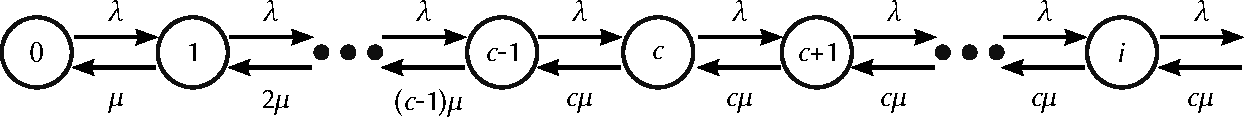
\includegraphics[width=\textwidth]{images/markovchain.pdf}
	\caption{$M/M/n-\infty$ Markov chain model.}
\label{c4:fig:markovchain}
\end{figure}

One such basic queuing system is $M/M/1-\infty$ \cite[pp.~94-99]{Kleinrock:1975:TVQ:1096491}, on which stationary analysis can be applied upon. Both the one processor queue and $M/M/n-\infty$ can also be easily expressed as a Markov chain due to their memoryless property. Figure~\ref{c4:fig:markovchain} depicts the state transitions of a system with $i$ processors and a queue length of $n-i$.

More complex models are often not tractable by stationary analysis or other mathematical tools any more and no general solution is known. This is especially true for the class of $G/G/n$ systems, which can only be directly solved under certain conditions. A better approach can be the use of a queuing simulation. Hereby, both the arrival and the serving process are implemented in a \gls{DES} using random numbers of the desired distributions in order to ascertain the system load and blocking probability.


%%%%%%%%%%%%%%%%%%%%%%%%%%%%%%%%%%%%%%%%%%%%%%%%%%%%%%%%%%%%%%%%%%%%%%%%%%%%%%%
\subsection{GGSN Model Rationale and General Queuing Theoretic Representation}

The \gls{GGSN} was already determined to be critical to the \gls{CN}'s load. Therefore, the network will be represented by this node in the model. Additionally, most of the load influencing factors are at least to a degree related to the \gls{gtp} tunnels. So, to dimension a mobile network to its control plane load, the number of supported tunnels have to be modeled. 


\begin{figure}[htb]
	\centering
	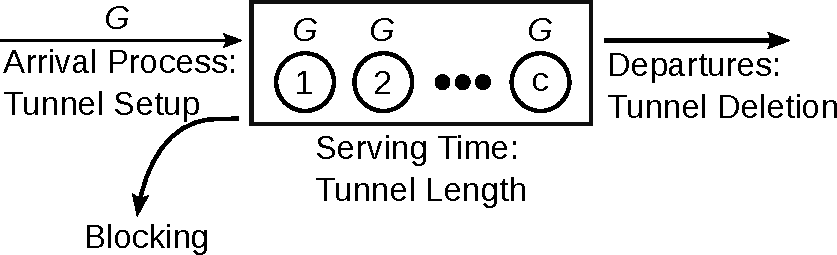
\includegraphics[width=\textwidth]{images/GGn-model.pdf}
	\caption{Queuing system representation of a mobile network's \gls{GGSN}.}
\label{c4:fig:ggn-model}
\end{figure}


Figure~\ref{c4:fig:ggn-model} shows this model for the proposed tunnel load metric and is in its generic form a $G/G/c-0$ system. Tunnels enter the system governed by a general random distribution and are served at the \gls{GGSN} for the duration of their existence. This duration also follows a general distribution. Afterwards, tunnels leave the system again through the reception of a \gls{gtp} tunnel delete message. If all $c$ serving units are filled, blocking occurs and arriving tunnel requests are rejected.

The number of serving units correspond to available resources at the \gls{GGSN}. The maximum supported number of concurrent tunnels is hard to estimate as it depends on a number of factors, most of which are unknown for this modeling process. This could include soft-limits like the specific configuration, and hard-limits, e.g. the \gls{GGSN}'s processing and memory constraints. 

For the purpose of creating an initial toy model the generic $G/G/c-0$ is simplified to a $M/M/\infty$ system. As stated, no actual limit to the number of virtual servers is known and the data also does not show any obvious limits. Thus, an unlimited system with neither blocking or queuing is assumed for this simple model.

Now, assuming both a Poisson arrival and an exponential serving process, a stationary analysis can be conducted. As seen in the statistical evaluation, the former condition may hold, but the serving time is definitely not exponentially distributed. However, for the toy model this assumption is still made to get an initial grasp of the model.

The diurnal influences seen in the tunnel arrivals in the trace data are also temporarily ignored and only the overall empirical distribution is taken into account. Through distribution fitting with moment matching the overall arrival rate is set to be $\lambda=25.64123$ in the trace. The exponential service time distribution is calculated to have the parameter $\mu=0.0001586728$. Using Little's Law this gives an estimate for the mean number of concurrent tunnels at the \gls{GGSN} in a $M/M/\infty$ system of 

\begin{equation}
\phantom{.}L=\frac{\lambda}{\mu}\approx 161.6\text{.} %=161598.14.
\end{equation}

As stated, the amount of state held at the node and propagated through the network is directly related to the number of tunnels. Therefore, this metric can serve as an initial estimate of the load at the \gls{GGSN}.


%%%%%%%%%%%%%%%%%%%%%%%%%%%%%%%%%%%%%%%%%%%%%%%%%%%%%%%%%%%%%%%%%%%%%%%%%%%%%%%
\subsection{Representative GGSN Models} 

With the experience from the toy model at hand more appropriate models can now be constructed to better accommodate for the core network's properties. Two models are provided here.
The first describes a monolithic version of a \gls{GGSN}, closely resembling the system used traditionally in the network. The second model is that of a hypothetical virtualized \gls{GGSN} using \gls{NFV}. In \gls{NFV}~\cite{nfv_whitepaper} monolithic network nodes are replaced by commodity hardware. The tasks solved by the original hardware is hereby migrated to software.


%%
\subsubsection{Monolithic \texorpdfstring{\acrshort{GGSN}}{GGSN}}

\begin{figure}[htb]
	\centering
	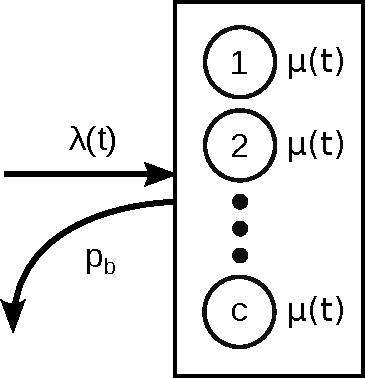
\includegraphics[width=0.5\textwidth]{images/ggsn-monolithic.pdf}
	\caption{Model of a Traditional GGSN}
\label{c4:fig:model-ggsn-monolithic}
\end{figure}

Traditionally, the \gls{GGSN} is considered to be one fixed entity, even if in reality it consists of multiple servers. The entire \gls{GGSN} is purchased from a vendor as a single entity, they do not integrate well with other existing network infrastructure. Nor can idle instances be deactivated or reused for other purposes.

The queuing theoretic equivalent is displayed in Figure~\ref{c4:fig:model-ggsn-monolithic} and is very similar to the basic toy model.
New tunnels requests arrive according to a Poisson distribution with a rate of $\lambda(t)$ at the \gls{GGSN}. The periodic time-of-day dependence of these exponentially distributed \gls{IAT} and the corresponding distribution fits were extrapolated from the trace data.

 will further have a maximum tunnel capacity of $c$. When this capacity is reached, blocking will occur and further incoming tunnels are rejected. The governing factors of the capacity are mostly the node's available memory and processing capabilities. Monolithic \glspl{GGSN} need to be preemptively dimensioned in such a way that blocking rarely happens, often resulting in gross overdimensioning as the node can not be easily scaled after it has been deployed.

When an incoming tunnel request is accepted one of the \gls{GGSN}'s serving units will be occupied for the tunnel's duration $x(t)$. Following the trace data, this duration is assumed to be of an arbitrary, albeit non-Markovian, service time distribution, again with a slight time-of-day dependence.
The empirical data was mapped with rational functions previously depicted in Table~\ref{c4:tab:fits}.

Together, this results in a \textbf{non-stationary Erlang loss model}, or more precisely

\begin{equation}
\phantom{.}M(t)/G(t)/c/0\text{.}
\end{equation}

With this model, high control plane load can be indirectly described as the system's blocking probability $p_B$. The peak load can be ascertained by looking at the busy hour period where the arrival rate is the highest. No exact solution is known for this type of model. Only if the service time distribution can be confined to certain specific distributions, e.g. Phase-type distributions, some approximations can be made \cite{davis1995nonstationaryerlang}. This confinement could not yet be made for the trace data. Instead, a simulative approach is taken in Section~\ref{c4:simulation}.


%%
\subsubsection{Virtualized \texorpdfstring{\acrshort{GGSN}}{GGSN}}
\label{c4:sec:virtual_ggsn}

\begin{figure}[htb]
	\centering
	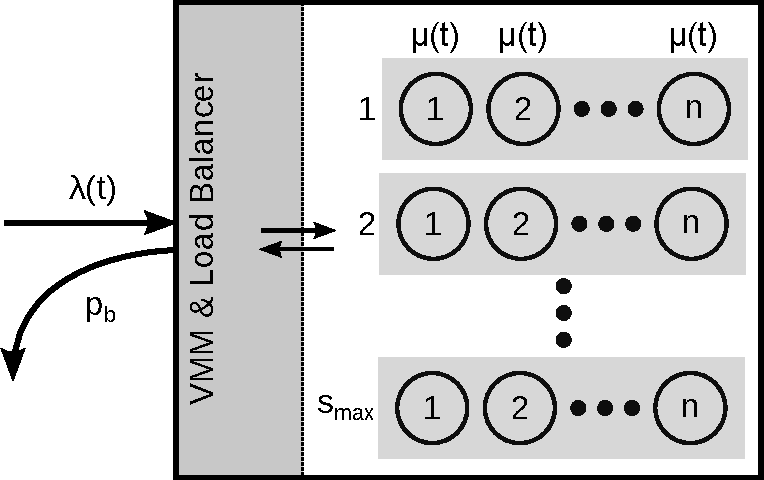
\includegraphics[width=0.8\textwidth]{images/ggsn-virtualized.pdf}
	\caption{Model of a GGSN using Network Function Virtualization}
\label{c4:fig:model-ggsn-virtualized}
\end{figure}

In the second model, virtualization concepts are introduced. The assumptions of the non-stationary Markov arrival process $\lambda(t)$ and the serving time distributions $x(t)$ are carried over. However, instead of one server processing every tunnel, the system is now partitioned into individual server instances coordinated by a load balancer in Figure~\ref{c4:fig:model-ggsn-virtualized}. One virtual \gls{GGSN} has up to $s$ servers instances $s_i$.  Each of the individual instances can be much smaller than the monolithic \gls{GGSN}, having a concurrent tunnel serving capacity of $c_i \ll c$ and a total system capacity of $c_{virt} = \sum_{i=1}^{s} c_i = \| \overrightarrow{c}\|_1 \text{ with } \overrightarrow{c} = \{c_1, c_2, ... ,c_i, ... ,c_s\}$. % 1-norm des Kapazitätsvektors
The complete model now reads:

\begin{equation}
\phantom{.}M(t)/G(t)/\|\overrightarrow{c}\|_1/0\text{.}
\end{equation}

The instances do not have a static uptime. Instead, their life cycle is managed by a \gls{VMM} and adjusted to the current load of the network. New tunnels are either placed on running instances or new ones are provisioned on demand. The \gls{VMM} can have multiple optimization goals. A prominent example is the minimization of server instance and energy usage.  Another set of example provisioning rules is discussed in the implementation of the model simulation in Section~\ref{c4:sec:eval_ideal_virtual_ggsn}. 

A target criterion could be to keep the blockinb probability inside a certain target range. If the \gls{VMM} decision rules are not carefully selected additional blocking could occur. Despite not having reached its maximum capacity, this system will still reject tunnel requests during the provisioning phase when no tunnel slots are free. This could be remedied by a request queue. However, this makes the system more complex without providing real benefit, as failed tunnel requests are retransmitted by the network control plane or another attempt might also be made directly by the mobile device after a timeout.

To place incoming tunnel state on one of the available servers and manage the servers a load balancer or hypervisor is required. To ensure, that the system can scale down to its actual needs, the balancer should place tunnels on servers, that are the fullest, keeping the reserve free. It may even migrate tunnel state from almost empty servers away so that these can be shut down, when certain conditions are fulfilled. Keeping instance close to their capacity should also have no impact on the performance a mobile device associated to a specific tunnel experiences. Adequate strategies for both load balancing and migration should be considered in subsequent research.

Through this virtualized model, which suggests to use technologies from cloud computing in the network and replace specialized nodes with commodity hardware, network operators can scale the \gls{GGSN} out instead of only up. Today, these network components are typically sold in a static and monolithic form and can not be easily extended with of-the-shelf hardware in order to accommodate to a changing environment. The system in this model can however be easily scaled out to additional low cost machines instead of completely replacing the existing \gls{GGSN} with a more powerful version. 

It is also entirely possible that the described single-arrival-process approaches might not the best way to describe control plane load. Several load influencing factors discussed earlier have direct influence on the tunnel arrivals and duration, e.g. the device type or the radio access technology. Therefore, amongst others, multidimensional queuing networks or fluid flow models could be more appropriate in subsequent research. But, the non-stationary Erlang loss model described here should be sufficient for basic core network control plane load estimations.

